\section{\rqthree}

The third research question investigates the impact of the composition of program variants into multivariant binaries.
To answer this research question, we create multivariant binaries out of the program variants generated for the \corpussodium and the \corpusqrcode corpora. We deploy the multivariant binaries into the Edge and we collect their function call traces and execution times.

This section is organized as follows ... 

\subsection*{Multivariant binary traces.}

We execute the multivariant binaries of each program, on the Fastly edge-cloud infrastructure. 
We execute each endpoint 100 times on each of the 64 edge nodes.
All the executions of a given endpoint are performed with the same input.
After each execution of an endpoint, we collect the sequence of invoked functions, i.e., the execution trace \todo{check name}. 


\begin{figure*}[h]
    \includegraphics[width=0.9\linewidth]{plots/rq3.3d.pdf}
    \caption{Ratio of unique execution traces for each endpoint on each edge node.   The X axis illustrates the edge nodes.
    The Y axis annotates the name of the endpoint.
    In the plot, for a given (x,y) pair, there is blue point representing the \autoref{metric:ratio:mve} value in a set of 100 collected execution traces.}
    \label{rq3:hashes:collision}
\end{figure*}

\autoref{rq3:hashes:collision} shows the ratio of unique traces exhibited by each endpoint, on each of the 64 separate edge nodes. 
The X corresponds to the edge nodes.
The Y axis gives the name of the endpoint.
In the plot, for a given (x,y) pair, there is blue point in the Z axis representing \autoref{metric:ratio:mve} over 100 execution traces.

% large spread and non-zero in all cases
For all edge nodes, the ratio of unique traces is above 0.38.
In 6 out of 7 cases, we have observed that the ratio is remarkably high, above 0.9.
These results show that we generate multivariant binaries that can randomize execution paths at runtime, in the context of an edge node. The composition of the variants, associated to a significant number of function variants greatly reduce the certainty about which computation is performed when running a specific input with a given input value.

Let's illustrate the phenomenon with the program \texttt{invert}.
The program \texttt{invert} receives a vector of integers and returns its inversion.
When the program is executed 100 times with the same input on the multivariant binary, we observe between 95 and 100 unique execution traces, depending on the edge node.
Analyzing the traces we observe that they include only two invocations the composition of variants for two different functions, one at the start of the trace and one at the end.
The remaining events in the trace are fixed each time the program is executed with the same input we provide in our experiments.
Thus, the maximum number of possible unique traces is the multiplication of the number of variants for each involved function, in this case $29\times96=2784$. The probability of observing the same trace is $1/2784$.


For multivariant binaries that embed only a few variants, like in the case of the \texttt{bin2base64} program, the ratio of unique traces per node is lower than for the other programs.
With the input we pass to \texttt{bin2base64}, the execution trace includes 57 function calls.
We have observed that this program selects among 41 variants of one diversified function. Thus,  probability of having the same execution trace  twice is $1/41$. 

Meanwhile, \texttt{qr\_str} embeds thousands of variants, and the input we pass triggers the invocation of 3M functions, for which 210666 random choices are taken relying on 17 variants' populations. Consequently, the probability of observing the same trace twice is minimal. Indeed, all the executions of \texttt{qr\_str} are unique, on each separate edge node.


We build the union of all the execution traces  collected on all edge nodes for a given program. 
Then, we compute the normalized Shannon Entropy over this set for each endpoint (\autoref{metric:entropy}).
Our goal is to determine whether the diversity of execution traces we previously observed on individual nodes, actually generalizes to the whole edge-cloud infrastructure. Depending on many factors, such as the random selection of variants during runtime, it could happen that we observe different traces on individual nodes, but that the set of traces is the same on all nodes.


The second column of \autoref{rq3:table:entropy} gives the normalized Shannon Entropy value (\autoref{metric:entropy}). Columns 3 and 4 give  the median and the standard deviation for the length of the execution traces. Columns 5 and 6 give 
the number of diversified function involved in the execution of the programs (\#Diversified) and the total number of invocations of these programs (\#Runtime choices). These last two columns indicate to what extent the execution paths are actually randomized at runtime. In the cases of \texttt{invert} and \texttt{random}, both have the same number of taken random choices. However, the number of variants to chose in \texttt{random}  are larger, thus, the entropy, is larger than \texttt{invert}.

\definecolor{celadon}{rgb}{0.67, 0.88, 0.69}
{
\begin{table}
%\setlength\minrowclearance{1.0pt}
\small
\centering
%\resizebox{\linewidth}{!}{
\begin{tabular}{  p{1.9cm} |  r | r r | r r }

    Endpoint & Entropy & Mean Trace Length & $\sigma$ & \#Diversified & \#Runtime choices \\
    \hline
    \hline
    
    \textbf{libsodium}  \\
    \hline
    
encrypt & 0.87 & 816 & 0 & 5  & 4M\\

decrypt & 0.96  & 440 & 0 & 5 & 2M\\

random & 0.98 & 15 & 5 & 2 & 12800\\

invert & 0.87  & 7343 & 0 & 2 & 12800\\

bin2base64 & 0.42  & 57 & 0 & 1 & 6400\\

\hline
\textbf{qrcode-rust} \\
\hline
qr\_str & 1.00 & 3045193 & 0 & 17 & 1348M \\
qr\_image & 1.00  & 3015450 & 0 & 15 & 1345M\\
\hline

\end{tabular}
%}
\caption{Execution trace diversity over the edge-cloud computing platform. The table is formed of 6 columns: the name of the program, the normalized Shannon Entropy value (\autoref{metric:entropy}), the median size of the execution traces, the standard deviation for the trace lengths the number of executed dispatchers (\#Diversified) and the number of total random choices taken during all the 6400 executions (\#Runtime choices).}\label{rq3:table:entropy}
\end{table}
}


Overall, the normalized Shannon Entropy (\autoref{metric:entropy}) is above 42\%. This is evidence that the multivariant binaries generated can indeed exhibit a high degree of execution trace diversity, while keeping the same functionality. The number of randomization points along the execution paths (\#Runtime choices) is at the core of these high entropy values. For example, every execution of the \texttt{encrypt} endpoint triggers 4M random choices among the different function variants embedded in the multivariant binaries. Such a high degree of randomization is essential to generate very diverse execution traces. 

The \texttt{bin2base64} endpoint has the lowest level of diversity. This endpoint is the one that has the least variants and its execution path can be randomized only at one function. The low level of unique traces observed on individual nodes is reflected at the system wide scale with a globally low entropy.

For both  \texttt{qr\_str} and \texttt{qr\_image} the entropy value is 1.0. This means that all the traces that we observe for all the executions of these endpoints are different from each other. In other words, someone who runs these services over and over with the same input cannot know exactly what code will be executed in the next execution.
These very high entropy values are made possible by the millions of random choices that are made along the execution paths of these endpoints.


% What is happening with the trace lengths
While there is a high degree of diversity among the traces exhibited by each endpoint, they all have the same length, except in the case of  \texttt{random}.
This means that the entropy is a direct consequence of randomly executing different function variants.
In the case of \texttt{random}, it naturally has a non-deterministic behavior.
Meanwhile, we observe several calls to variants composition in during the execution of the multivariant binary, which indicates that \tool can amplify the natural diversity of traces exhibited by \texttt{random}. 
For each endpoint, we managed to trigger all dispatchers during its execution.


\subsection*{Execution times.}

For each program, we compare the execution time distributions for the original binary and the multivariant binary. All distributions are measured on 100k executions.
% statistics
We have observed that the distributions for multivariant binaries  have a higher standard deviation of execution time.
A statistical comparison between the execution time distributions confirms the significance of this difference (P-value = 0.05 with a  Mann-Withney U test). This hints at the fact that  the execution time for multivariant binaries is more unpredictable than the time to execute the original binary. 

% Curve flatenning
In \autoref{rq3:diversity:times}, each subplot represents the distribution for a single program, with the colors blue and green representing the original and multivariant binary respectively. These plots reveal  that the execution times are indeed spread over a larger range of values compared to the original binary. 
This is evidence that execution time is less predictable for multivariant binaries than for the original ones.

\begin{figure*}[h]
    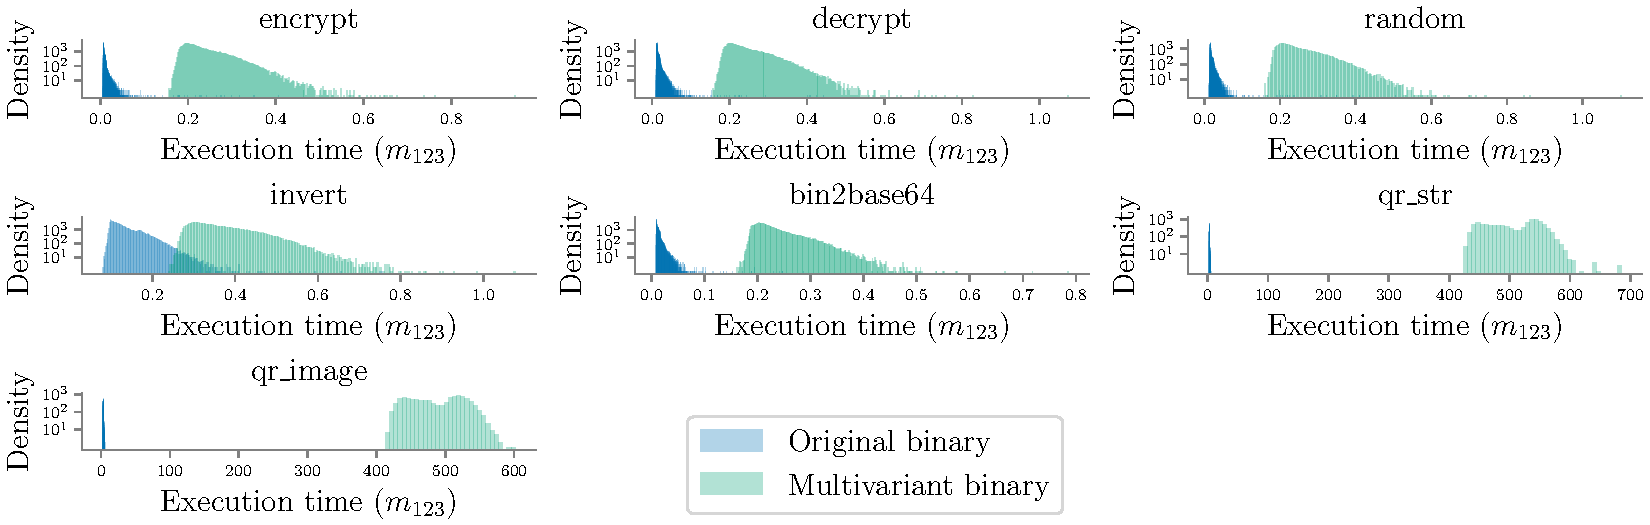
\includegraphics[width=\linewidth]{plots/times.pdf}
    \caption{Execution time distributions. Each subplot represents the distribution for a single program, blue for the original program and green for the multivariant binary. The X axis shows the execution time in milliseconds and the Y axis shows the density distribution in logarithmic scale.}
    \label{rq3:diversity:times}
\end{figure*}


Recall that the choice of function variant is randomized at each function invocation, and the variants have different execution times as a consequence of the code transformations, i.e., some variants execute more instructions than others. 
Consequently, attacks relying on measuring precise execution times of a function are made a lot harder to conduct as the distribution for the multivariant binary is different and even more spread than the original one.

\section{Answer to RQ3.}


Repeated executions of a multivariant binary with the same input on an individual edge node exhibits diverse execution traces.
\tool successfully synthesizes multivariant binaries that trigger diverse execution paths at runtime, on individual edge nodes. 


At the internet scale of the Edge platform, the multivariant binaries synthesized by \tool exhibit a massive diversity of execution traces, while still providing the original service.
It is virtually impossible for an attacker to predict which is taken for a given query.



The execution time distributions are significantly different between the original and the multivariant binary. Furthermore, no specific variant can be inferred from execution times gathered from the multivariant binary. \tool contributes to mitigate potential attacks based on predictable execution times.